\documentclass[12pt]{beamer}

\usepackage[english]{babel}
\usepackage[T1]{fontenc}
\usepackage[utf8]{inputenc}
\usepackage{enumitem, tikz, chronosys}

\usetikzlibrary{patterns}

\setitemize{
  itemsep=1em,
  label=\usebeamerfont*{itemize item}
    \usebeamercolor[fg]{itemize item}
    \usebeamertemplate{itemize item}
}

\usetikzlibrary{positioning, decorations.markings}
\tikzset{small/.style={draw,fill,circle,inner sep=1pt,outer sep=0pt}}

\setbeamertemplate{footline}[frame number]{}
\setbeamertemplate{navigation symbols}{}

% https://tex.stackexchange.com/a/167423
\newcommand{\backupbegin}{
  \newcounter{framenumberappendix}
  \setcounter{framenumberappendix}{\value{framenumber}}
}
\newcommand{\backupend}{
  \addtocounter{framenumberappendix}{-\value{framenumber}}
  \addtocounter{framenumber}{\value{framenumberappendix}}
}

\title{Reduction of Key Sizes on Rainbow-like Multivariate Signature Schemes}
\author{Gustavo Zambonin}
\institute{
  \includegraphics[scale=0.15]{ufsc}                        \\
  Qualification Exam                                        \\
  Graduate Program in Computer Science                      \\ \vspace{2mm}
  \texttt{gustavo.zambonin@posgrad.ufsc.br}
}
\date{}

\begin{document}

\begin{frame}[plain,noframenumbering]
  \titlepage{}
\end{frame}

\begin{frame}
  \frametitle{Context}
  \begin{itemize}
    \item Guarantee protection and privacy of messages sent digitally
    \item Security of digital signature schemes is based on problems from
        number theory
    \begin{itemize}
      \item Integer factorization, discrete logarithm
    \end{itemize}
    \item There exist quantum algorithms~\cite{Shor:article:1997:oct} that
        solve such problems efficiently
    \item Post-quantum cryptography aims to create cryptosystems based on
        problems immune to quantum speed-ups
  \end{itemize}
\end{frame}

\begin{frame}
  \frametitle{Motivation}
  \begin{itemize}
    \item Foreshadowing of quantum computers
    \item Several active branches of post-quantum cryptography based on
        distinct mathematical structures
    \item Standardization calls by institutions such as NIST, IRTF and ETSI
    \item We focus on cryptosystems that are built upon the difficulty of
        solving systems of equations
  \end{itemize}
\end{frame}

\begin{frame}
  \frametitle{Multivariate cryptography}
  \begin{itemize}
    \item Cryptography based on systems of multivariate quadratic equations
        over finite fields
    \item Bipolar construction:
    \begin{figure}
      \vspace{2mm}
      \centering
      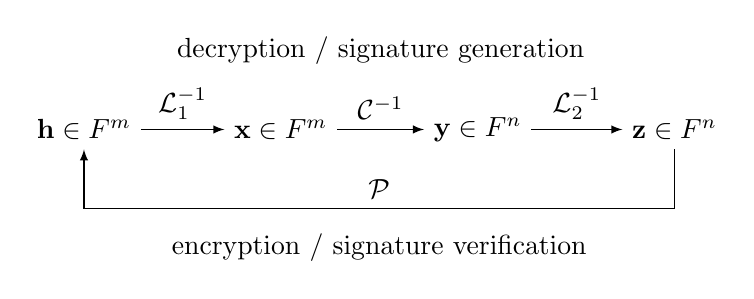
\begin{tikzpicture}
        \node (h) at (-2.5, 0) {$\mathbf{h} \in \mathbb{F}^{m}$};
        \node (x) at (0, 0) {$\mathbf{x} \in \mathbb{F}^{m}$};
        \node (y) at (2.5, 0) {$\mathbf{y} \in \mathbb{F}^{n}$};
        \node (z) at (5, 0) {$\mathbf{z} \in \mathbb{F}^{n}$};
        \draw[-latex] (h) -- (x) node[midway,above] {$\mathcal{L}_{1}^{-1}$};
        \draw[-latex] (x) -- (y) node[midway,above] {$\mathcal{C}^{-1}$}
          node[midway,yshift=1cm] {decryption / signature generation};
        \draw[-latex] (y) -- (z) node[midway,above] {$\mathcal{L}_{2}^{-1}$};
        \draw[-latex] (z) -- (5, -1) -- (-2.5, -1) node[midway,above]
          {$\mathcal{P}$} node[midway,yshift=-.5cm] {encryption / signature
          verification} -- (h);
      \end{tikzpicture}
    \end{figure}
    \item Fast operations, small signature sizes and large keys, compared to
        conventional schemes
  \end{itemize}
\end{frame}

\begin{frame}
  \frametitle{Research object}
  \begin{itemize}
    \item Focus on the Rainbow signature scheme~\cite{Ding:inproc:2005:jun},
        currently on Round 2 of the NIST standardization process
    \item Easy description, good balance between signature and key sizes
    \item Keys are one to two orders of magnitude greater than
        conventional ones
    \item Generalized version of Unbalanced Oil and
        Vinegar~\cite{Kipnis:inproc:1999:apr}
  \end{itemize}
\end{frame}

\begin{frame}
  \frametitle{Related works}
  \begin{figure}[htbp]
    \tiny
    \vspace{-1.5cm}
    \startchronology[startyear=2010,stopyear=2020,dates=false,arrow=false,height=3pt]
    \definechronoevent{sp}[datesseparation=/, conversionmonth=false]
    \chronosp[colorbox=blue!10,markdepth=-50pt]{06/2010}{\cite{Petzoldt:inproc:2010:jun}*}
    \chronosp[colorbox=blue!20]{12/2010}{\cite{Petzoldt:inproc:2010:dec}}
    \chronosp[colorbox=blue!30,markdepth=-20pt]{03/2011}{\cite{Petzoldt:inproc:2011:mar}*}
    \chronosp[colorbox=blue!30,markdepth=40pt]{09/2011}{\cite{Petzoldt:inproc:2011:sep}}
    \chronosp[colorbox=red!20,markdepth=-50pt]{02/2012}{\cite{Yasuda:inproc:2012:feb}$\dagger$}
    \chronosp[colorbox=blue!40,markdepth=40pt]{11/2012}{\cite{Petzoldt:inproc:2012:nov}}
    \chronosp[colorbox=red!30]{5/2013}{\cite{Yasuda:inproc:2013:may}*}
    \chronosp[colorbox=blue!20,markdepth=-50pt]{06/2013}{\cite{Petzoldt:inproc:2013:jun}}
    \chronosp[colorbox=blue!40,markdepth=-20pt]{07/2013}{\cite{Petzoldt:phd:2013:jul}}
    \chronosp[colorbox=red!30,markdepth=40pt]{04/2014}{\cite{Yasuda:inproc:2014:apr}*}
    \chronosp[colorbox=red!40,markdepth=-20pt]{09/2014}{\cite{Yasuda:article:2014:sep}*}
    \chronosp[colorbox=blue!30]{12/2015}{\cite{Shim:inproc:2015:dec}}
    \chronosp[colorbox=red!40,markdepth=-50pt]{06/2017}{\cite{Peng:article:2017:jun}$\dagger$}
    \chronosp[colorbox=blue!20]{06/2017}{\cite{Szepieniec:inproc:2017:jun}}
    \chronosp[colorbox=blue!20,markdepth=-20pt]{12/2017}{\cite{Beullens:inproc:2017:dec}}
    \chronosp[colorbox=purple!50]{05/2019}{Ours}
    \stopchronology \vspace{.5cm}
    {\scriptsize
      Works in blue optimise public keys, while red ones reduce private keys.
      Asterisks denote reparametrized works and crosses denote broken schemes.
    }
  \end{figure}
\end{frame}

\begin{frame}
  \frametitle{Hypothesis}
  \begin{itemize}
    \item To the best of our knowledge, works have reduced either private or
        public keys
    \item Introduction of structures in the keys may lower security
  \end{itemize}
  \vspace{1cm}
  \begin{itemize}
    \item \textbf{Can both reductions be achieved simultaneously}?
  \end{itemize}
\end{frame}

\begin{frame}
  \frametitle{Rainbow signature scheme}
  \framesubtitle{Preliminaries}
  \begin{itemize}
    \item Parameters are a finite field $\mathbb{F}_{q}$, integers $u, n$ such
        that $u \leq n$ and $0 < v_{1} < \cdots < v_{u} < v_{u + 1} = n$
    \item For $1 \leq \ell \leq u$, set vinegar variables
        $V_{\ell} = \{1, \dots, v_{\ell}\}$ and oil variables
          $O_{\ell} = \{v_{\ell} + 1, \dots, v_{\ell + 1}\}$
    \item Define vector spaces spanned by quadratic Oil-Vinegar polynomials
    \begin{align*}
      P_{\ell} = \sum_{i, j \in V_{\ell}} \alpha_{ij}  x_{i}  x_{j}
        + \sum_{i \in V_{\ell}, j \in O_{\ell}} \beta_{ij}  x_{i}  x_{j}
        + \sum_{i \in V_{\ell} \cup O_{\ell}} \gamma_{i}  x_{i} + \delta, \\
        \alpha_{ij}, \beta_{ij}, \gamma_{i}, \delta \in \mathbb{F}_{q}
    \end{align*}
  \end{itemize}
\end{frame}

\begin{frame}
  \frametitle{Rainbow signature scheme}
  \framesubtitle{Key generation}
  \begin{itemize}
    \item Let $m = n - v_{1}$ and $o_{\ell} = v_{\ell + 1} - v_{\ell}$
    \item Randomly pick two affine transformations
        $\mathcal{L}_{1} : \mathbb{F}_{q}^{m} \to \mathbb{F}_{q}^{m}$ and
        $\mathcal{L}_{2} : \mathbb{F}_{q}^{n} \to \mathbb{F}_{q}^{n}$
    \item Central map is a function
        $\mathcal{C} : \mathbb{F}_{q}^{n} \to \mathbb{F}_{q}^{m}$
      \begin{itemize}
        \item A total of $o_{\ell}$ polynomials and respective coefficients are
            randomly chosen from each $P_{\ell}$
      \end{itemize}
    \item Private key is the $3$-uple
        $(\mathcal{L}_{1}, \mathcal{C}, \mathcal{L}_{2})$, public key is the
          composition $\mathcal{P} = \mathcal{L}_{1} \circ \mathcal{C} \circ
          \mathcal{L}_{2}$
  \end{itemize}
\end{frame}

\begin{frame}
  \frametitle{Rainbow signature scheme}
  \framesubtitle{Inversion of the central map}
  \begin{itemize}
    \item Vinegar variables of a layer are exactly the oil and vinegar
        variables from the previous layer
    \item This enables the inversion of each Oil-Vinegar layer recursively
    \item With $u = 2$, the initial configuration of $\mathcal{C}$ is
        \vspace{.25cm}
    \begin{figure}
      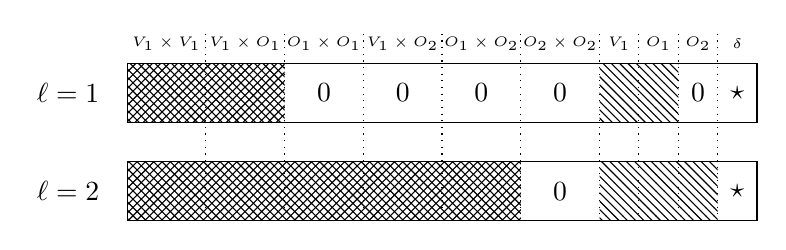
\begin{tikzpicture}
        \node (v1v1) at (0.5, 1) {\tiny $V_{1} \times V_{1}$};
        \node (v1o1) at (1.5, 1) {\tiny $V_{1} \times O_{1}$};
        \node (o1o1) at (2.5, 1) {\tiny $O_{1} \times O_{1}$};
        \node (v1o2) at (3.5, 1) {\tiny $V_{1} \times O_{2}$};
        \node (o1o2) at (4.5, 1) {\tiny $O_{1} \times O_{2}$};
        \node (o2o2) at (5.5, 1) {\tiny $O_{2} \times O_{2}$};
        \node (v1)   at (6.25, 1) {\tiny $V_{1}$};
        \node (o1)   at (6.75, 1) {\tiny $O_{1}$};
        \node (o2)   at (7.25, 1) {\tiny $O_{2}$};
        \node (l)    at (7.75, 1) {\tiny $\delta$};
        \foreach \r in {1, ..., 6, 6.5, 7, 7.5}
          \draw[dotted] (\r, 1.125) to (\r, -1.25);

        \draw (0, 0) rectangle (8, 0.75);
        \node (l1)   at (-0.75, 0.375) {$\ell = 1$};
        \fill[pattern=crosshatch] (0, 0) rectangle (2, 0.75);
        \fill[pattern=north west lines] (6, 0) rectangle (7, 0.75);
        \foreach \r in {2.5, ..., 5.5} \node at (\r, 0.375) {$0$};
        \node (o2c1)  at (7.25, 0.375) {$0$};
        \node (lc1)  at (7.75, 0.375) {$\star$};

        \draw (0, -0.5) rectangle (8, -1.25);
        \node (l1)   at (-0.75, -0.875) {$\ell = 2$};
        \fill[pattern=crosshatch] (0, -0.5) rectangle (5, -1.25);
        \fill[pattern=north west lines] (6, -0.5) rectangle (7.5, -1.25);
        \node (o2c2) at (5.5, -0.875) {$0$};
        \node (lc2)  at (7.75, -0.875) {$\star$};
      \end{tikzpicture}
    \end{figure}
  \end{itemize}
\end{frame}

\begin{frame}
  \frametitle{Rainbow signature scheme}
  \framesubtitle{Inversion of the central map}
  \begin{itemize}
    \item Randomly choose variables in $V_{1}$ and substitute them
          \vspace{.25cm}
    \begin{figure}
      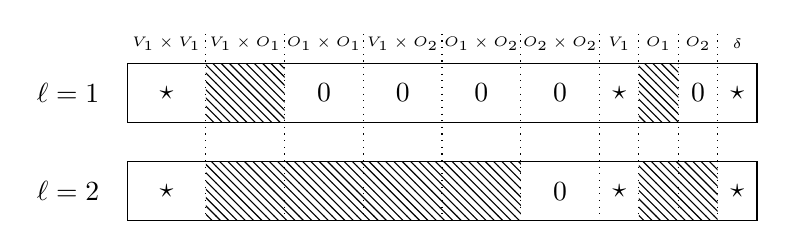
\begin{tikzpicture}
        \node (v1v1) at (0.5, 1) {\tiny $V_{1} \times V_{1}$};
        \node (v1o1) at (1.5, 1) {\tiny $V_{1} \times O_{1}$};
        \node (o1o1) at (2.5, 1) {\tiny $O_{1} \times O_{1}$};
        \node (v1o2) at (3.5, 1) {\tiny $V_{1} \times O_{2}$};
        \node (o1o2) at (4.5, 1) {\tiny $O_{1} \times O_{2}$};
        \node (o2o2) at (5.5, 1) {\tiny $O_{2} \times O_{2}$};
        \node (v1)   at (6.25, 1) {\tiny $V_{1}$};
        \node (o1)   at (6.75, 1) {\tiny $O_{1}$};
        \node (o2)   at (7.25, 1) {\tiny $O_{2}$};
        \node (l)    at (7.75, 1) {\tiny $\delta$};
        \foreach \r in {1, ..., 6, 6.5, 7, 7.5}
          \draw[dotted] (\r, 1.125) to (\r, -1.25);

        \draw (0, 0) rectangle (8, 0.75);
        \node (l1)   at (-0.75, 0.375) {$\ell = 1$};
        \fill[pattern=north west lines] (1, 0) rectangle (2, 0.75);
        \fill[pattern=north west lines] (6.5, 0) rectangle (7, 0.75);
        \foreach \r in {2.5, ..., 5.5, 7.25} \node at (\r, 0.375) {$0$};
        \foreach \r in {0.5, 6.25, 7.75} \node at (\r, 0.375) {$\star$};

        \draw (0, -0.5) rectangle (8, -1.25);
        \node (l1)   at (-0.75, -0.875) {$\ell = 2$};
        \fill[pattern=north west lines] (1, -0.5) rectangle (5, -1.25);
        \fill[pattern=north west lines] (6.5, -0.5) rectangle (7.5, -1.25);
        \foreach \r in {0.5, 6.25, 7.75} \node at (\r, -0.875) {$\star$};
        \node at (5.5, -0.875) {$0$};
      \end{tikzpicture}
    \end{figure}
    \item Solve linear $o_{1}$ equations in the first layer to obtain $V_{2}$,
        and then solve the remaining $o_{2}$ equations \vspace{.25cm}
    \begin{figure}
      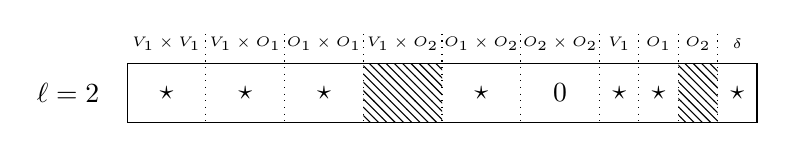
\begin{tikzpicture}
        \node (v1v1) at (0.5, 1) {\tiny $V_{1} \times V_{1}$};
        \node (v1o1) at (1.5, 1) {\tiny $V_{1} \times O_{1}$};
        \node (o1o1) at (2.5, 1) {\tiny $O_{1} \times O_{1}$};
        \node (v1o2) at (3.5, 1) {\tiny $V_{1} \times O_{2}$};
        \node (o1o2) at (4.5, 1) {\tiny $O_{1} \times O_{2}$};
        \node (o2o2) at (5.5, 1) {\tiny $O_{2} \times O_{2}$};
        \node (v1)   at (6.25, 1) {\tiny $V_{1}$};
        \node (o1)   at (6.75, 1) {\tiny $O_{1}$};
        \node (o2)   at (7.25, 1) {\tiny $O_{2}$};
        \node (l)    at (7.75, 1) {\tiny $\delta$};
        \foreach \r in {1, ..., 6, 6.5, 7, 7.5}
          \draw[dotted] (\r, 1.125) to (\r, 0);

        \draw (0, 0) rectangle (8, 0.75);
        \node (l2)   at (-0.75, 0.375) {$\ell = 2$};
        \fill[pattern=north west lines] (3, 0) rectangle (4, 0.75);
        \fill[pattern=north west lines] (7, 0) rectangle (7.5, 0.75);
        \foreach \r in {0.5, ..., 2.5, 4.5, 6.25, 6.75, 7.75}
          \node at (\r, 0.375) {$\star$};
        \node at (5.5, 0.375) {$0$};
      \end{tikzpicture}
    \end{figure}
  \end{itemize}
\end{frame}

\begin{frame}
  \frametitle{Rainbow signature scheme}
  \framesubtitle{Signature generation}
  \begin{itemize}
    \item Consider a cryptographic hash function
        $\mathcal{H} : \{0, 1\}^{*} \to \mathbb{F}_{q}^{m}$ and a message $M$,
          and compute the digest $\mathbf{d} = \mathcal{H}(M)$
    \item Obtain the value $\mathbf{x} = \mathcal{L}_{1}^{-1}(\mathbf{d})$
    \item Generate the pre-image of $\mathbf{x}$ under the central map,
        $\mathbf{y} = \mathcal{C}^{-1}(\mathbf{x})$, as per the operations
          above
    \item Compute the final signature
        $\mathbf{z} = \mathcal{L}_{2}^{-1}(\mathbf{y})$
  \end{itemize}
\end{frame}

\begin{frame}
  \frametitle{Rainbow signature scheme}
  \framesubtitle{Signature verification}
  \begin{itemize}
    \item Obtain $\mathbf{d}$ from the message $M$
    \item Compute $\mathbf{d}' = \mathcal{P}(\mathbf{z})$
    \item The signature is valid if $\mathbf{d} = \mathbf{d}'$, and invalid
        otherwise
  \end{itemize}
\end{frame}

\begin{frame}
  \frametitle{Our proposal}
  \begin{itemize}
    \item Introduction of structures in the private key is dangerous and may
        lead to security holes
    \item Observe that, to invert the central map, vinegar variables are
        chosen randomly every time a preimage is computed
    \item If these variables are changed less often, or fixed, they simplify
        the central map matrix representation
    \item Indeed, the central map may be stored in a linearized fashion, and
        regenerated only occasionally
  \end{itemize}
\end{frame}

\begin{frame}
  \frametitle{Our proposal}
  \begin{itemize}
    \item We propose to fix the $V_{1}$ variables throughout the central map
    \item A possible implementation of this method is to use a PRNG to
        regenerate $\mathcal{C}$ every time it is needed
    \item The linear relations described in
        CyclicRainbow~\cite{Petzoldt:inproc:2010:dec} are another way to obtain
        the original central map
    \item The EUF-CMA variant described in~\cite{Ding:misc:2017:dec} provides
        a salt that can be modified instead of vinegar variables
  \end{itemize}
\end{frame}

\begin{frame}
  \frametitle{Our proposal}
  \begin{itemize}
    \item Only variables in $V_{1}$ are fixed, since $V_{2}$ and beyond need
        the digest to be calculated
    \item Strategy is not hindered by current cryptanalytic methods, since the
        choice of parameters does not change
    \item General framework for every Rainbow-like scheme
    \item Can be applied on top of variants that reduce the public key,
        confirming our hypothesis
  \end{itemize}
\end{frame}

\begin{frame}
  \frametitle{Open problems}
  \begin{itemize}
    \item Given multiple signatures created with the same set of vinegar
        variables, is it possible to unveil information about the private key?
    \item Does every signature needs its own set of vinegar variables or is the
        cost of regenerating the central map amortized?
    \item Is it possible to create a constant-time implementation with this
        strategy?
    \item Do there exist parameter sets which optimize the private key size?
  \end{itemize}
\end{frame}

\backupbegin{}
\begin{frame}[plain, allowframebreaks]
  \frametitle{References}
  \bibliographystyle{alpha}
  {\scriptsize \bibliography{\jobname}}
\end{frame}
\backupend{}

\end{document}
